\documentclass[a4paper, 12pt]{article}

\usepackage[portuges]{babel}
\usepackage[utf8]{inputenc}
\usepackage{amsmath}
\usepackage{indentfirst}
\usepackage{graphicx}
\usepackage[colorinlistoftodos]{todonotes}

\usepackage{listings}
\lstset{language=Fortran,
             basicstyle=\footnotesize,
             numbers=left,
             numberstyle=\footnotesize,
             frame=shadowbox,
             rulesepcolor=\color{blue}}



%\input logo

%\vspace*{-3cm}

%\begin{figure}[h]
%\leavevmode
%\begin{minipage}[t]{\textwidth}
%\includegraphics[1cm,1cm][3cm,3cm]{logo-ufrpe.bmp}
%\end{minipage}
%\end{figure}

\begin{document}
%\maketitle

\begin{titlepage}
	\begin{center}
	{\large
		\hspace*{0cm}Universidade Federal de Juiz de Fora} \\
        \hspace*{0cm}Departamento de Ciência da Computação \\
        \hspace*{0cm}DCC059 - Teoria dos Grafos Semestre 2016-3  \\

\vspace{10pt}

        
        \vspace{85pt}
        
		\textbf{\LARGE{Trabalho da Disciplina de Grafos}}
		\vspace{160pt}
		
	\end{center}
	
	\begin{flushleft}
		\begin{tabbing}
			Alunos\qquad\qquad\= Bruno José Cesário de Almeida Martins\\
			\> Cláudio Nazareth Lopes\\
            \> Gabriell Lucas Ribeiro Medeiros\\
            \> Lucas Paiva Bressan \\
			Professor\> Stênio Sã Rosário F. Soares \\
		
	\end{tabbing}
		  
	\end{flushleft}
	
	\begin{center}
		\vspace{\fill}
		\vspace{2cm}
			{\center Juiz de Fora \\[3mm]
			Dezembro de 2016 \\}
	\end{center}
\end{titlepage}
%%%%%%%%%%%%%%%%%%%%%%%%%%%%%%%%%%%%%%%%%%%%%%%%%%%%%%%%%%%
\newpage
\tableofcontents
\thispagestyle{empty}

\newpage
\pagenumbering{arabic}

%%%%%%%%%%%%%%%%%%%%%%%%%%%%%%%%%%%%%%%%%%%%%%%%%%%%%%%%%
%%%%%%%%%%%%%%%%%%%%%%%%%%%%%%%%%%%%%%%%%%%%%%%%%%%%
\section{Introdução}

Este trabalho tem como objetivo desenvolver funções algorítmicas estudadas em sala de aula para resolvermos problemas da área de Grafos e apresentar uma heurística para o problema do Corte Mínimo de Vértices.
\\ \\ \indent Um Corte Mínimo de Vértices se dá pelo menor número de nós que podem ser removidos de um grafo que aumentem o número de suas componentes conexas em 1. Este problema é muito importante caso por exemplo, desejamos testar
o quão conexa uma rede é (podendo esta rede ser uma rede de computadores, rede elétrica ou rede de telefonia...). Através dele conseguimos descobrir, no caso de uma rede de telefonia, quantas antenas em uma certa área devem falhar para que o sinal de celular seja interrompido por exemplo.
\section{Metodologia utilizada}

Para os testes dos algoritmos utilizados neste trabalho, foram usadas instâncias passadas pelo professor da disciplina. Dentre estas, haviam vários modelos dos quais somente alguns foram selecionados para a realização de testes de funcionamento e a tentativa de obter-se um boa solucão a partir da heurística proposta. A escolha das instâncias foi baseada no número total de arestas de cada uma, portanto quanto maior o número de arestas, maior esta instância é considerada.

\subsection{Estruturas de dados utilizadas}

Para a representação dos Grafos nós utilizamos a estrutura Lista de Adjacência. Os códigos foram programados na linguagem C++.
\subsection{Abordagens algorítmicas usadas na solução}
Para melhor entendimento do algoritmo, são explicadas abaixo as funcionalidades do Grafo proposto como trabalho.
\subsubsection{Incluir e excluir nó e aresta}
Para  operação de inclusão de um nó a função recebe como parâmetro um (id) e o cria no grafo. Na operação de inclusão de uma aresta, a função recebe como parâmetro dois (ids) de vértices diferentes cria a aresta entre os dois e caso um dos ids não esteja no grafo (grafo não direcionado), a função o cria.

Para operação de exclusão de nós a função recebe como parâmetro um (id) e o deleta juntamente com todas as arestas ligadas a ele. Já na exclusão de uma aresta, a função recebe como parâmetro dois ids de vértices e deleta, caso exista, a aresta que liga os dois vértices.

\subsubsection{Retornar o grau de nó passado no parâmetro}

A função recebe como parâmetro um id de um vértice contido no grafo. É feito uma contagem de quantos vértices são adjacentes ao vértice parâmetro e retorna esse valor.

\subsubsection{Retornar a sequência de graus do grafo}
Essa função cria um array de tamanho igual ao número de nós. Obtém-se todos os graus de nós do grafo e que em seguida é ordenado por outra função. A função retorna um vetor em ordem decrescente dos graus dos nós obtidos.

\subsubsection{Verificar se  o grafo é k-regular}
Essa função cria um nó auxiliar para percorrer todo grafo. É criado um inteiro que recebe o grau do primeiro nó armazenado no grafo e em seguida e comparado com todos os graus dos nós restantes no grafo. A função retorna 0 (zero) caso o grau de algum nó seja diferente do primeiro obtido. A função retorna K, sendo esse K um número inteiro positivo, com o valor do grau do primeiro nó obtido na função, sendo este o K-Regularidade do grafo.

\subsubsection{Verificar se o grafo é completo}
Essa função cria um nó auxilar para percorrer todo o grafo. Este auxilar recebe o grau do vértice obtido onde é comparado se é menor que o número total de vértices menos um. Se a afirmação for verdadeira a função retorna um booleano falso, caso contrário a função retorna um booleano verdadeiro, dizendo que o grafo é completo.

\subsubsection{Verificar se dois nós são adjacentes}
A função recebe como parâmetro dois ids de vértices do grafo. É criado dois nós auxilares para que recebem esses ids. Se um dos ids for nulo ou seja não está no grafo, a função retorna um booleano falso. Caso eles existam é feito uma busca na lista de adjacência de cada vértice pedido pela função e obtêm-se como resultado um booleano verdadeiro caso exista adjacência nas duas listas. Caso contrário é retornado um booleano falso.


\subsubsection{Busca em largura e profundidade}
Para a função de Busca em Largura a função recebe como parâmetro um id de um vértice contido no grafo. É criado dois vetores (v1) que armazena a sequencia, (v2) que armazena o vértices visitados. No início a função coloca na pilha (v2) o vértice passado como parâmetro e cria um nó auxiliar (n1) para percorrer todo grafo. A função executa laço buscando todos os vértices alcançados a partir daquele vértice e caso chegue em algum que não se liga a outro vértice que está na solução, a função retorna para um vértice que consiga alcançar outro vértice que ainda não está na solução. A execução termina quando todos os vértices alcançáveis a partir do vértice parâmetro está na solução que é armazenado em (v1). A função retorna (v1).  

Para a função de Busca em Profundidade a função recebe como parâmetro um id de um vértice contido no grafo. É criado três vetores (v1) que armazena a busca, (v2) que faz o papel de uma pilha e (v3) que contém os vértices visitados. No início insere o vértice parâmetro no final (v2), cria um vértice auxiliar (n1), um outro vetor (v4) que faz interações no grafo e um inteiro (k) com vértice atual. Em seguida é executado um laço de repetição que pega o nó atual e insere em (v1) e (v3). Insere no (v2) todos os nós adjacentes a posição (k) no vetor (v2). Logo apos remove (k) do vetor (v2). O laço termina quando a pilha estiver vazia, ou seja (v2) vazio e (v1) com todos os vértices do grafo na ordem que foram obtidos.

\subsubsection{Verificar se o grafo é conexo}
É criado um vetor de inteiros que armazena o vetor obtido na busca em largura. A função retorna um booleano verdadeiro caso o tamanho do vetor obtido seja igual a quantidade de vértices do grafo. Caso contrário é retornado um booleano falso.

\subsubsection{Verificar se dois nós estão em uma mesma componente conexa}
A função recebe como parâmetro dois ids de vértices contidos no grafo. São criados três vetores (v1, v2, v3) de inteiros onde o primeiro (v1) armazena o vetor obtido na busca em largura do grafo. O segundo (v2) armazena uma busca dentro do primeiro vetor obtido procurando o primeiro id passado com parâmetro. O terceiro (v3) também armazena uma busca dentro do primeiro vetor procurando o segundo id passado como parâmetro. Se na busca dos dois vetores (v2 e v3) conterem os ids passados com parâmetro a função retorna um booleano verdadeiro dizendo que os dois vértices pertencem a uma mesma componente conexa. Caso contrário a função retorna um booleano falso. 

\subsubsection{Verificar se um dado nó é de articulação}
A função recebe como parâmetro um id de um dado nó do grafo. É criado um grafo auxilar idêntico ao grafo original. É feito uma busca por um nó fonte do grafo que é armazenado em um nó auxiliar criado (n1). Cria-se um vetor de inteiros (v1) que armazena uma busca em profundidade a partir de (n1). Em seguida é deletado do grafo o vértice obtido por parâmetro. Novamente é feito uma busca por um nó fonte do grafo e armazenado em (n1). Cria-se um novo vetor (v2) que guarda uma busca em profundidade a partir de (n1). A função retorna um booleano falso caso o tamanho de (v1) seja igual ao tamanho de (v2) mais (+) 1(um). Caso contrário a função retorna um booleano verdadeiro dizendo que o nó é de articulação.

\subsubsection{Verificar se uma dada aresta é ponte}
A função recebe como parâmetro dois ids de vértices do grafo. Cria um grafo auxiliar idêntico ao grafo original e um nó auxiliar (n1) que armazena um nó ponte do grafo. Cria um vetor (v1) o qual armazena um busca em profundidade a partir de (n1). Em seguida é deletado a aresta que liga os dois vértices passados como parâmetro e na sequência é feita uma nova busca por um nó fonte no grafo onde é armazenado (n1). Cria um no vetor (v2) onde o mesmo armazena uma busca em profundidade a partir de (n1). A função retorna um booleano falso caso o tamanho de (v1) seja igual ao tamanho de (v2), caso contrário a função retorna um booleano verdadeiro dizendo que a aresta em questão é uma aresta ponte.

\subsubsection{Retornar a vizinhança (aberta/fechada) de um dado nó}
Para a vizinhança aberta a função recebe como parâmetro um id de algum nó do grafo e cria um no (n1) auxiliar que obtém a busca do primeiro nó da sua lista de adjacência. É criado um vetor (v1) de inteiros do tamanho do grau de (n1). É feito um laço para obter todos os nós da lista de adjacência de (n1) e armazená-los em (v1). A função retorna (v1).

Para a vizinhança fechada a função recebe como parâmetro um id de algum nó do grafo e cria um no (n2) auxiliar que é igual ao id passado. Se (n2) for nulo então a função retorna um erro. Caso não seja nulo a função cria um vetor (v2) de tamanho do grau do vértice mais um. Cria-se um laço para obter a lista de adjacência do (n2) e armazena-la em (v2). A função retorna (v2). 

\subsubsection{Retornar o fechamento transitivo direto/indireto de um dado nó}
Para o fecho transitivo direto a função recebe como parâmetro um id de um nó contido no grafo. Caso o grafo não seja um dígrafo a função retorna um erro. Caso seja um dígrafo a função cria um vetor (v1) para armazenar todo o fecho direto. Em seguida aplica-se a função da Matriz de Floyd (m1) e executado um laço para determinar os vértices dentro desta matriz na posição onde se encontra o vértice recebido por parâmetro. Todo posição de vértice dentro da matriz que incide no nó passado por parâmetro e armazenado em (v1). A final da execução a função retorna um o vetor (v1) contendo o fecho transitivo direto.

Para o fecho transitivo indireto a função recebe como parâmetro um id de um nó contido no grafo. Caso o grafo não seja um dígrafo a função retorna um erro. Caso seja um dígrafo a função cria um vetor (v1) para armazenar todos os vértices que entraram no fecho transitivo indireto. Em seguida é aplicado a função para se obter a Matriz de Floyd (m1). Logo após é executado um laço de repetição para saber todos os vértices em que o vértice passado por parâmetro incide. Esses vértices são guardados dentro de (v1). Ao final da execução a função retorna (v1).

\subsubsection{Retornar a ordenação topológica do DAG}
A função cria três vetores (v1), (v2) e (v3), onde (v1) vai armazenar a ordenação topológica do grafo, (v2) armazena todos os nós fontes do grafo e (v3) armazena somente um elemento (-1) que significa que o grafo não é uma DAG. É criado um  grafo auxiliar (g1) que é idêntico ao grafo original e também é criado um nó auxiliar (n1) que armazena o primeiro nó do grafo. É feito um laço de repetição onde é armazenado em (v2) todos os nos fontes do grafo. Logo em seguida é criado outro laço de repetição é atualizado a (v2) até que o mesmo seja vazio, armazena em (v1) o DAG do grafo e ao longo das interações são retiradas arestas de (g1). A função retorna (v3) se o número de arestas de (g1) for maior que 0 (zero). Caso contrário a função retorna (v1) contendo a ordenação topológica do grafo em questão.

\subsubsection{Determinar o caminho mínimo entre dois vértices usando algoritmo de Dijkstra}
A função recebe como parâmetro dois ids (n1 e n2)) de vertices contidos no grafo. Primeiramente é feito um teste para verificar se vértices pertencem a mesma componente conexa, se não são, retorna um erro. Caso sejam da mesma componente conexa é criado dois vetores (v1) que armazena caminho e um vetor de vetores (v2) o qual armazena os nós não visitados. No início  a função atribui o valor zero para a distância do primeiro vértice a ele mesmo e para os demais seta a distância como infinito para nó origem. Em seguida a função entra num laço de repetição até que todos os vértices de(v2) estejam em (v1). Em cada interação a função escolhe o vértice de menor caminho entre (n1) e um dos nós contidos em (v2). Juntamente com isso a distância entre o (n1) e o vértice escolhido pela função são alterados. Ao final a função retorna o vetor (v1) que contém o menor caminho entre (n1) e (n2).

\subsubsection{Determinar o caminho mínimo entre qualquer par de vértices usando o algoritmo de Floyd}
A função cria uma matriz tridimensional de vetores (m1) e um vetor de vetores (m2) com a distâncias entre vértices. Ao longo de um laço de repetição (v1) é atualizado com a distância  de um determinado vértice a outro. Logo após a saída deste laço, a função entra em um outro, fazendo a atualização deste dados verificando se a distância de um dado elemento da matriz, que está representado por (m2), existi ou é infinito. Se existir a função atualiza está distância. Ao fim a função executa um laço montado a matriz (m1) através dos dados obtidos em (m2), a qual contém a distância de um determinado vértice para qualquer outro vértice contido no grafo.

\subsubsection{Retornar o subgrafo induzido por um dado subconjunto de vértices}
A função recebe como parâmetro um vetor de vértices contidos no grafo. Cria um novo grafo (g1) que é idêntico a grafo em questão e é criado também vetor (v2) que contém todos os vértices a serem removido do grafo. A função entra em um laço de repetição escolhendo os vértices que serão excluídos do grafo e os adicionando em (v2). A fim deste laço é executado um outro laço de repetição que pega todos os vértices contidos em (v2) e os excluí do grafo (g1). Formando assim o subgrafo obtido pelo vetor passado como parâmetro. A função retorna (g1).

\subsubsection{Retornar as componentes conexas do grafo}
A função cria um vetor de vetores (v1) que contém as componentes conexas do grafo. Cria também um vetor (v2) que contém o caminho da busca em largura a partir do primeiro vértice do grafo e cria um inteiro k que armazena o número de componente conexas do grafo. O índice zero do vetor (v1) contém (v2). Em seguida a função entra em um laço de repetição no qual faz uma busca pelas componentes conexas contidas no grafo e armazena em (v1) todos os caminhos destas componentes. Ao final da execução a função retorna (v1) onde está contida todas as componentes conexas do grafo.

\subsubsection{Retornar o grafo gerado pelo produto cartesiano entre o grafo e outro grafo}
A função recebe como parâmetro um grafo (g1) e cria um novo grafo (g2). A função entra em laço de repetição percorrendo o grafo recebido como parâmetro e o grafo da função, fazendo o produto cartesiano entre os dois. Ao longo desta interação é feito o somatório dos pesos das arestas que serão inseridos no novo grafo (g2) juntamente com o seus respectivos vértices obtidos no produto cartesiano. Ao final a função retorna (g2).

\subsubsection{Retornar a árvore geradora mínima usando o algoritmo de PRIM}
A função executa um teste para verificar se o grafo é dígrafo e caso a resposta seja verdadeira a função retorna um erro. Caso a execução continue a função cria um novo grafo (g1). O algoritmo seleciona um vértice contido no grafo e cada interação ele acrescenta a menor aresta incidente no conjunto de vértices que já foi selecionado e que possuí uma extremidade em vértices fora desse conjunto. Ao término da execução o algoritmo retorna o grafo (g1) o qual foi criado ao longo das interações onde foram encontrados o conjuntos de vértices.

\subsubsection{Retornar a árvore geradora mínima usando o algoritmo de Kruskal}
A função executa um teste para verificar se o grafo é dígrafo e caso a resposta seja verdadeira a função retorna um erro. Essa função trata como cada vértice do grafo com uma arvore independente. Ao longo das interações o algoritmo vai juntando essas arvores com menor peso de aresta que ligue uma arvore a outra. O algoritmo vai criando arvores que se obtenha uma floresta a qual é representada por um grafo (g1) que é construído ao longo da interações. A final de toda a execução a função retorna o grafo (g1) contendo a árvore geradora mínima.

\subsubsection{Verificar se o grafo é k-conexo}
A função recebe como parâmetro um inteiro k. É criado um vetor de vértices (v1) e um nó auxiliar para percorrer o grafo. Logo em seguida é criado um vetor de permutações (v2) o qual contém todas as K permutações possíveis do grafo. Logo após é criado um grafo (g1) para ser trabalhado nas interações que vai remover de k em k vértices e checará se o grafo continua conexo ou não. Caso em algumas da interações o grafo for desconexo a função retorna um booleano falso. Caso as interações terminem e o grafo (g1) continue conexo a função retorna um booleano verdadeiro o que significa que o grafo é k-conexo.

\subsubsection{Verificar se o grafo é euleriano}
A função cria um nó auxiliar (n1) para percorrer no grafo. É executado um teste para ver se o grafo é conexo e caso a resposta seja falsa ou seja o grafo é desconexo então a função retorna um booleano falso. Caso seja verdadeiro o teste então a função executa um laço percorrendo os vértices verificando se o grau deles é par. Se algum deles a resposta for ímpar a função retorna um booleano falso, caso contrário a função retorno um booleano verdadeiro, o que significa que o grafo é euleriano.

\subsection{Heuristica utilizada para segunda parte do experimento}
Na heurística utilizada ordena-se o grafo pelo grau de seus vertices e escolhe-se o vértice de menor grau. Em seguida, uma lista de candidatos é criada. Esta lista será composta por todos os vértices vizinhos ao vértice de menor grau escolhido e será ordenada do vertice de maior para o de menor grau. Após isso, entramos em uma estrutura de repetição em que cada iteração, o vértice de maior grau da lista de candidatos é excluído da lista e do grafo (na abordagem gulosa). Logo após verifica-se se o grafo ficou desconexo e assim até a lista de candidatos ficar vazia ou até o grafo se tornar desconexo. Caso o grafo fique desconexo após a remoção de um vertice, retornamos uma lista com este vertice mais os vertices removidos antes dele. Um dos principais motivos pelos quais escolhemos tal heuristica se dá pelo fato de que, ao pegar o vértice de menor grau de todo o grafo, tem-se a certeza de que um corte desse grafo pode ser menor ou igual ao grau deste vértice escolhido.

\subsection{Algorítimo Guloso}
 
 \begin{lstlisting} 
   getCorteGuloso (Grafo g) {
      a = getVerticeMenorGrau(g); 
      candidatos = getVizinhos(a); 
      ordenaCandidatos();
      solucao = {};
      num_componentes_original = g.getNumComponentes(); 
      i = 0;
      while (candidatos.size() != 0) {
         solucao.push_back(candidatos[i]);
          g.deletaVertice(candidatos[i]);
          num_componentes_atual = g.getNumComponentes(); 
          if (num_componentes_original != num_componentes_atual){
              return solucao;
          }
          i++;
      }
      return solucao;
   }
 \end{lstlisting}

\subsection{Algorítimo Guloso Randomizado}

\begin{lstlisting} 
   getCorteGulosoRandomizado(Grafo g, float alfa, int iteracoes) {
      while (iteracoes--) {
          a = getVerticeMenorGrau(g); 
          candidatos = getVizinhos(a); 
          ordenaCandidatos(); 
          do {
              index = xrandomRange(0, candidatos.size() * alfa);
              solucao.push_back(candidatos[index]);
              g.deletaVertice(candidatos[index]);
             atualizaCandidatos(index); 
          } while (candidatos.size() != 0);
          if (solucao.size() < best.size()) {
              best = solucao;
              solucao = {};
          }
      }
      return best;
   }
 \end{lstlisting}

\subsection{Algorítimo Guloso Randomizado Reativo}

\begin{lstlisting} 
   getCorteGulosoRandomizadoReativo(Grafo g) {
        iteracao = 25;
        alphas = [0.05, 0.1, 0.15, 0.2, 0.25, 
                0.3, 0.35, 0.4, 0.45, 0.5];
        
        for(int i=0; i<quantAlphas; i++){
            iteracoes.push_back(iteracao);
        }
    
        //O algoritmo roda 30 vezes
        for(int j=0; j<30; j++){
            media = 0;
        
            //roda o algoritmo randomizado para cada alpha
            for(int i=0; i<alphas.size(); i++){
            
                randomizado = corteVerticesGulosoRandomizado(g,
                            alphas[i],iteracoes[i],nomeArquivo);
            
                resultadosIteracoes[i].swap(randomizado);
            
            /* verifica se o tamanho do algoritmo randomizado
            é menor que a solucao atual*/
                if(randomizado.size() < melhoresSolucoes[i].size()
                    || melhoresSolucoes[i].size() == 0) {
                    melhoresSolucoes[i].swap(randomizado);
            }
        
            //pega o tamanho das soluções e faz um somatório
            for(int i=0; i<alphas.size(); i++){
                media += resultadosIteracoes[i].size();
            }
        
            /*refaz o numero de iterações para cada alpha
            tido como base quanto menor o tamanho da
            solucao maior o numero de iteracoes*/
            for(int i=0; i<alphas.size(); i++){
                iteracoes[i] =  
                (1-(resultadosIteracoes[i].size()/)media)) / 
                (alphas.size()-1))*iteracao*alphas.size()));
            }
            media = 0;
        }
    
        /*define a solução final como a menor solução
        entre as soluções encontradas usando os alphas*/
        for(int i=0; i<quantAlphas; i++){
            if(verticesCorte.size() > melhoresSolucoes[i].size()
                || verticesCorte.size() == 0)
                verticesCorte.swap(melhoresSolucoes[i]);
        }
        
        return verticesCorte;
   }
 \end{lstlisting}

\section{Experimentos Computacionais}

O ambiente de testes utilizado foi um computador com processador modelo Intel Core i5 de 2.4GHz com 8GB DDR3 de memória rodando o macOS 10.12.1. Para as instâncias médias e grandes na abordagem reativa nós também utilizamos um computador
com processador AMD A10 7850K de 4GHz com 8GB DDR3 de memória rodando o Ubuntu 16.04.
\\ \\ \indent Como já dito no item 2. deste documento, as instâncias escolhidas foram classificadas como pequenas, médias ou grandes
a partir da quantidade de arestas de cada uma. Todas as instâncias utilizadas neste primeiro teste se encontram na pasta \textbf{Instancias Grafos} junto ao código entregue com este documento e são elas:

\begin{itemize}
  \item \textbf{Instancias Pequenas:} grafo\_1000\_4.txt (14370 arestas), grafo\_1000\_8.txt (9983 arestas), grafo\_10000\_8.txt (10075 arestas), grafo\_10000\_4.txt (14588 arestas)
  \item \textbf{Instancias Medias:} grafo\_10000\_3.txt (58259 arestas), grafo\_1000\_3.txt (54990 arestas), grafo\_10000\_7.txt (42858 arestas)
  \item \textbf{Instancias Grandes:} grafo\_1000\_6.txt (109243 arestas), grafo\_10000\_6.txt (122847 arestas), grafo\_10000\_2.txt (159464 arestas)
\end{itemize}



\\ \\ \indent Na figura 1 (na sessão 5. Anexos) apresentamos uma tabela com os resultados obtidos apartir dos testes realizados sobre as instâncias escolhidas:
\\ \\ \ident Na primeira porção da imagem, vemos na primeira coluna, o nome de cada instância testada. Na segunda coluna temos o melhor valor de corte encontrado entre todas as execuções de todas as abordagens (gulosa, randomizada e reativa). Na terceira coluna nós temos o desvio da média da abordagem gulosa em relação ao melhor resultado obtido{\tiny*}, na quarta o desvio da média da abordagem randomizada e na quinta o desvio da média da abordagem reativa{\tiny*}.
\\ \\ \indent Na tabela ``Tempo Médio'' nós vemos o tempo médio que cada uma das abordagens demorou para serem executadas.
\\ \\ \indent Já na última tabela, nós temos a mesma tabela da primeira porção da imagem porém com a segunda coluna representando menor valor de corte possivel (não conseguimos obter o valor ótimo para todas as instâncias. Somente para aquelas que tinham como vertice de menor grau, um nó de grau 1 pois daí sabemos que o corte mínimo de um grafo com vértice de menor grau igual à 1 é 1 e um corte deste tamanho, é o menor corte possível em qualquer grafo que tenha um vértice destes).
\\ \\ \indent Os logs de cada uma das heuristicas testadas utilizando o nosso código neste primeiro teste estão na pasta \textbf{Resultados/Resultados do Trabalho - Teste 01}. Foi criado um arquivo para cada uma das abordagens (gulosa, gulosa randômica e gulosa randômica reativa), e são eles:
\begin{itemize}
  \item \textbf{Abordagem Gulosa:} guloso\_out\_original.txt
  \item \textbf{Abordagem Gulosa Randomizada:} guloso\_rand\_out\_original.txt
  \item \textbf{Abordagem Gulosa Randomizada Reativa:} guloso\_rand\_reativo\_out\_original.txt
\end{itemize}
\\ \\ {\tiny * Para obtermos a média, somamos o (melhor) resultado final de cada uma das 30 iterações e depois dividimos este valor por 30. Após, para encontrarmos o desvio fazemos  \( \frac{média - valor\_ótimo}{valor\_ótimo} \)} \\ \\

\ident Logo após rodarmos os testes decritos acima e notarmos que não seria possível executar o algorítimo reativo com todos os 10 alfas em um tempo hábil, decidimos testar a nossa heurística em instâncias menores. As instâncias selecionadas para este segundo teste foram todas encontradas em \\ \\ \textbf{https://turing.cs.hbg.psu.edu/txn131/graphcoloring.html} \\ \\Nós utilizamos novamente como parâmetro para definir se uma instância é pequena, média ou grande, o seu número de vértices. Como neste link, todas as instâncias foram usadas para o problema de coloração mínima de vértices, nós não temos o valor do menor corte de vértices possível para cada uma delas. 
\\ \\ \indent Todas as instâncias utilizadas neste segundo teste se encontram na pasta \textbf{Instancias02} junto ao código entregue com este documento e são elas:

\begin{itemize}
  \item \textbf{Instancias Pequenas:} pequena01 (11,20).txt (20 arestas), pequena02 (23,71).txt (71 arestas), pequena03 (37,72).txt (72 arestas), pequena04 (20,20).txt (20 arestas)
  \item \textbf{Instancias Medias:} media01 (100,166).txt (166 arestas), media02 (88,146).txt (146 arestas), media03 (79,156).txt (156 arestas)
  \item \textbf{Instancias Grandes:} grande01 (87,406).txt (406 arestas), grande02 (138,493).txt (493 arestas), grande03 (149,541).txt (541 arestas)
\end{itemize}

\\ \\ \indent Na figura 2 (na sessão 5. Anexos) apresentamos uma tabela identica a tabela da figura 1 porém com os resultados obtidos a partir do segundo teste realizado sobre as novas instâncias selecionadas. \\

\indent Os logs de cada uma das heuristicas testadas utilizando o nosso código neste segundo teste estão na pasta \textbf{Resultados/Resultados do Trabalho - Teste 02}. Foi criado um arquivo para cada uma das abordagens (gulosa, gulosa randômica e gulosa randômica reativa), e são eles:
\begin{itemize}
  \item \textbf{Abordagem Gulosa:} guloso\_out\_original.txt
  \item \textbf{Abordagem Gulosa Randomizada:} guloso\_rand\_out\_original.txt
  \item \textbf{Abordagem Gulosa Randomizada Reativa:} guloso\_rand\_reativo\_out\_original.txt
\end{itemize}

\section{Conclusões}
De acordo com os testes realizados em nosso primeiro teste, as funcionalidades se comportaram de maneira esperada, encontrando-se soluções satisfatórias que muitas das vezes, foram iguais ao menor corte possível (1). Tanto a heurística gulosa quanto a gulosa randomizada (utilizando alpha igual à 0.25 e número de iterações igual à 5) apresentaram soluções e tempo de execução satisfatórios para todas as instâncias escolhidas.
\\ 
\\
\ident Embora a abordagem gulosa randomizada reativa tenha apresentado resultados e tempo satisfatórios para as 
quatro Instâncias Pequenas escolhidas, seu desempenho em relação ao tempo de execução não foi muito bom para as instâncias médias e grandes. Desta forma, a única maneira que conseguimos rodar a abordagem reativa em todas as instancias foi ou reduzindo o número de alphas que o algorítimo testa ou diminuindo o número de iterações que ele faz por teste (e mesmo assim sua execução ficou lenta para as instâncias maiores porém seus resultados foram satisfatórios muitas das vezes, encontrando-se até a solução ótima). Não foi possível executar todas as 30 iterações na instância \textbf{grafo\_1000\_6.txt} uma vez que esta possuia vértices de graus muito grandes e demorava aproximadamente 30 minutos para cada uma das 30 vezes que ele rodava (usando somente 5 alphas e 4 como o número de iterações) o algorítimo \textbf{Guloso Randômico Reativo.} \\

\ident Já no segundo teste, como trabalhamos com instâncias menores, nós conseguimos obter tanto soluções quanto tempos de execução satisfatórios para todas as instâncias nas heurísticas gulosa, gulosa randômica (utilizando alpha igual à 0.25 e número de iterações igual à 15) e gulosa randomizada reativa (utilizando dez alphas diferentes e 75 iterações para cada uma das 30 vezes que nós rodamos o algorítimo ranômico para cada um dos dez alphas).

\section{Anexos}

  \begin{figure}[h]
    \centering
    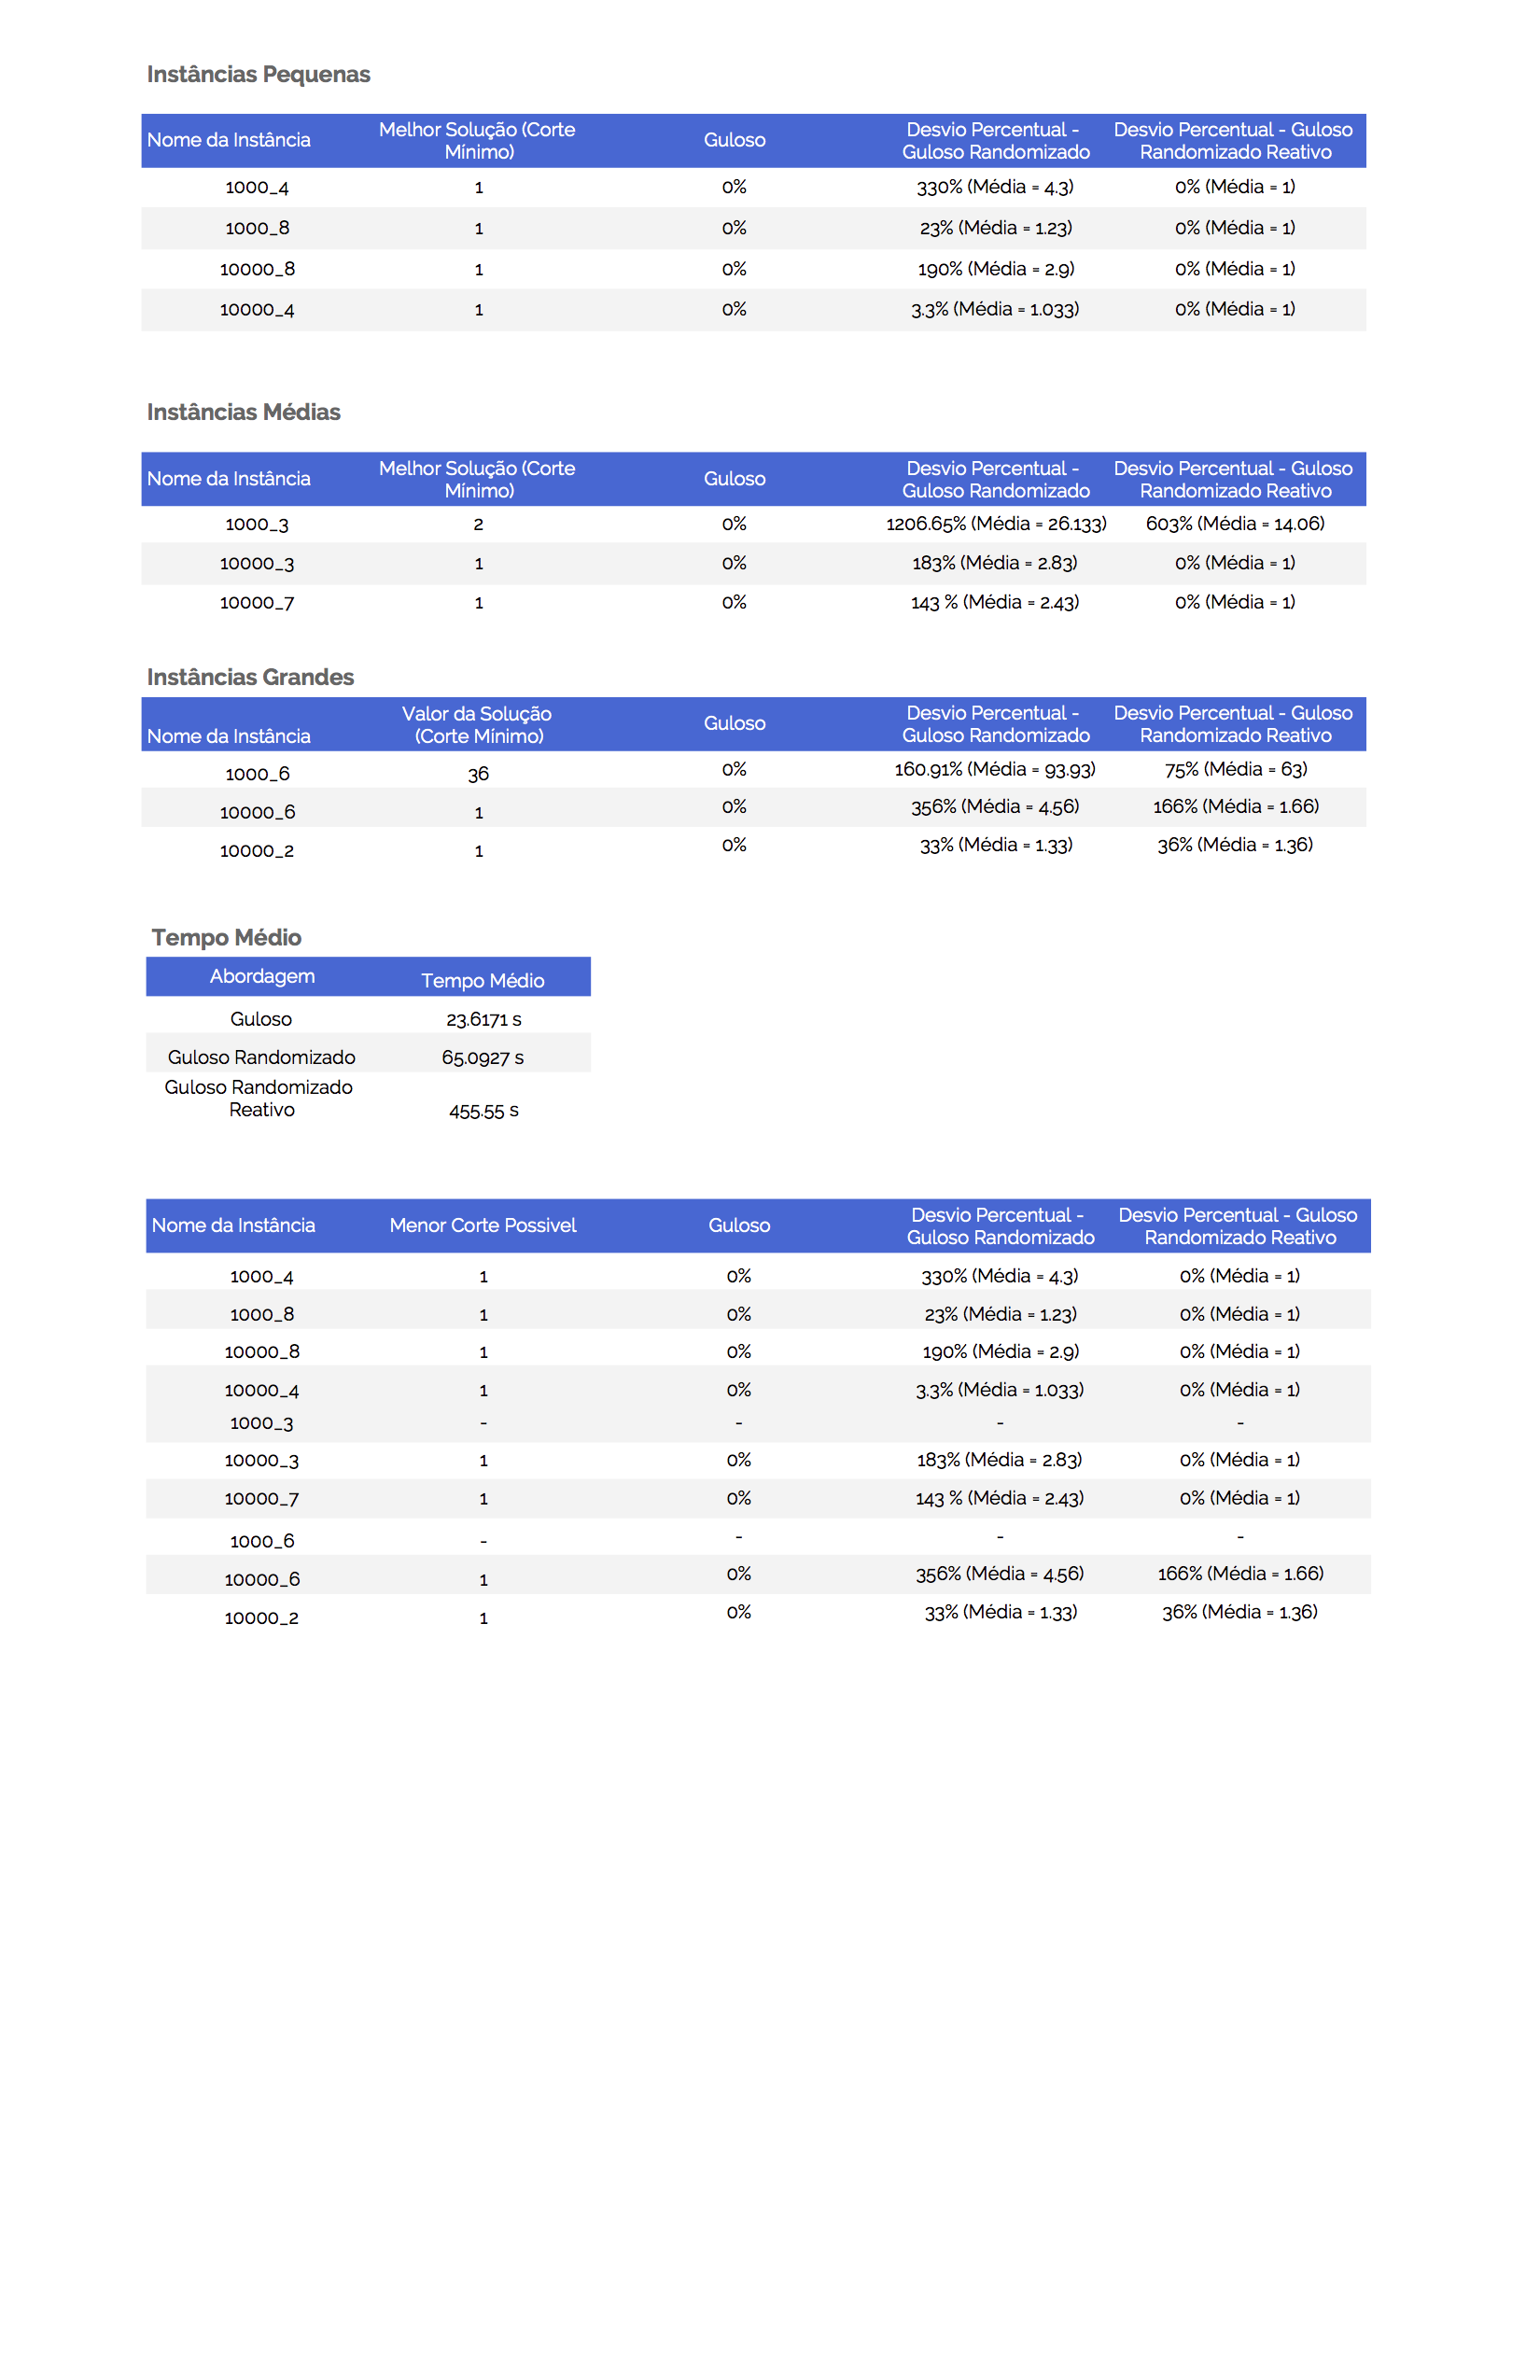
\includegraphics[width=14cm, height = 20cm]{TabelaResultados}
    \caption{Tabela de com resultados obtidos no primeiro teste }
  \end{figure}

  \begin{figure}[h]
    \centering
    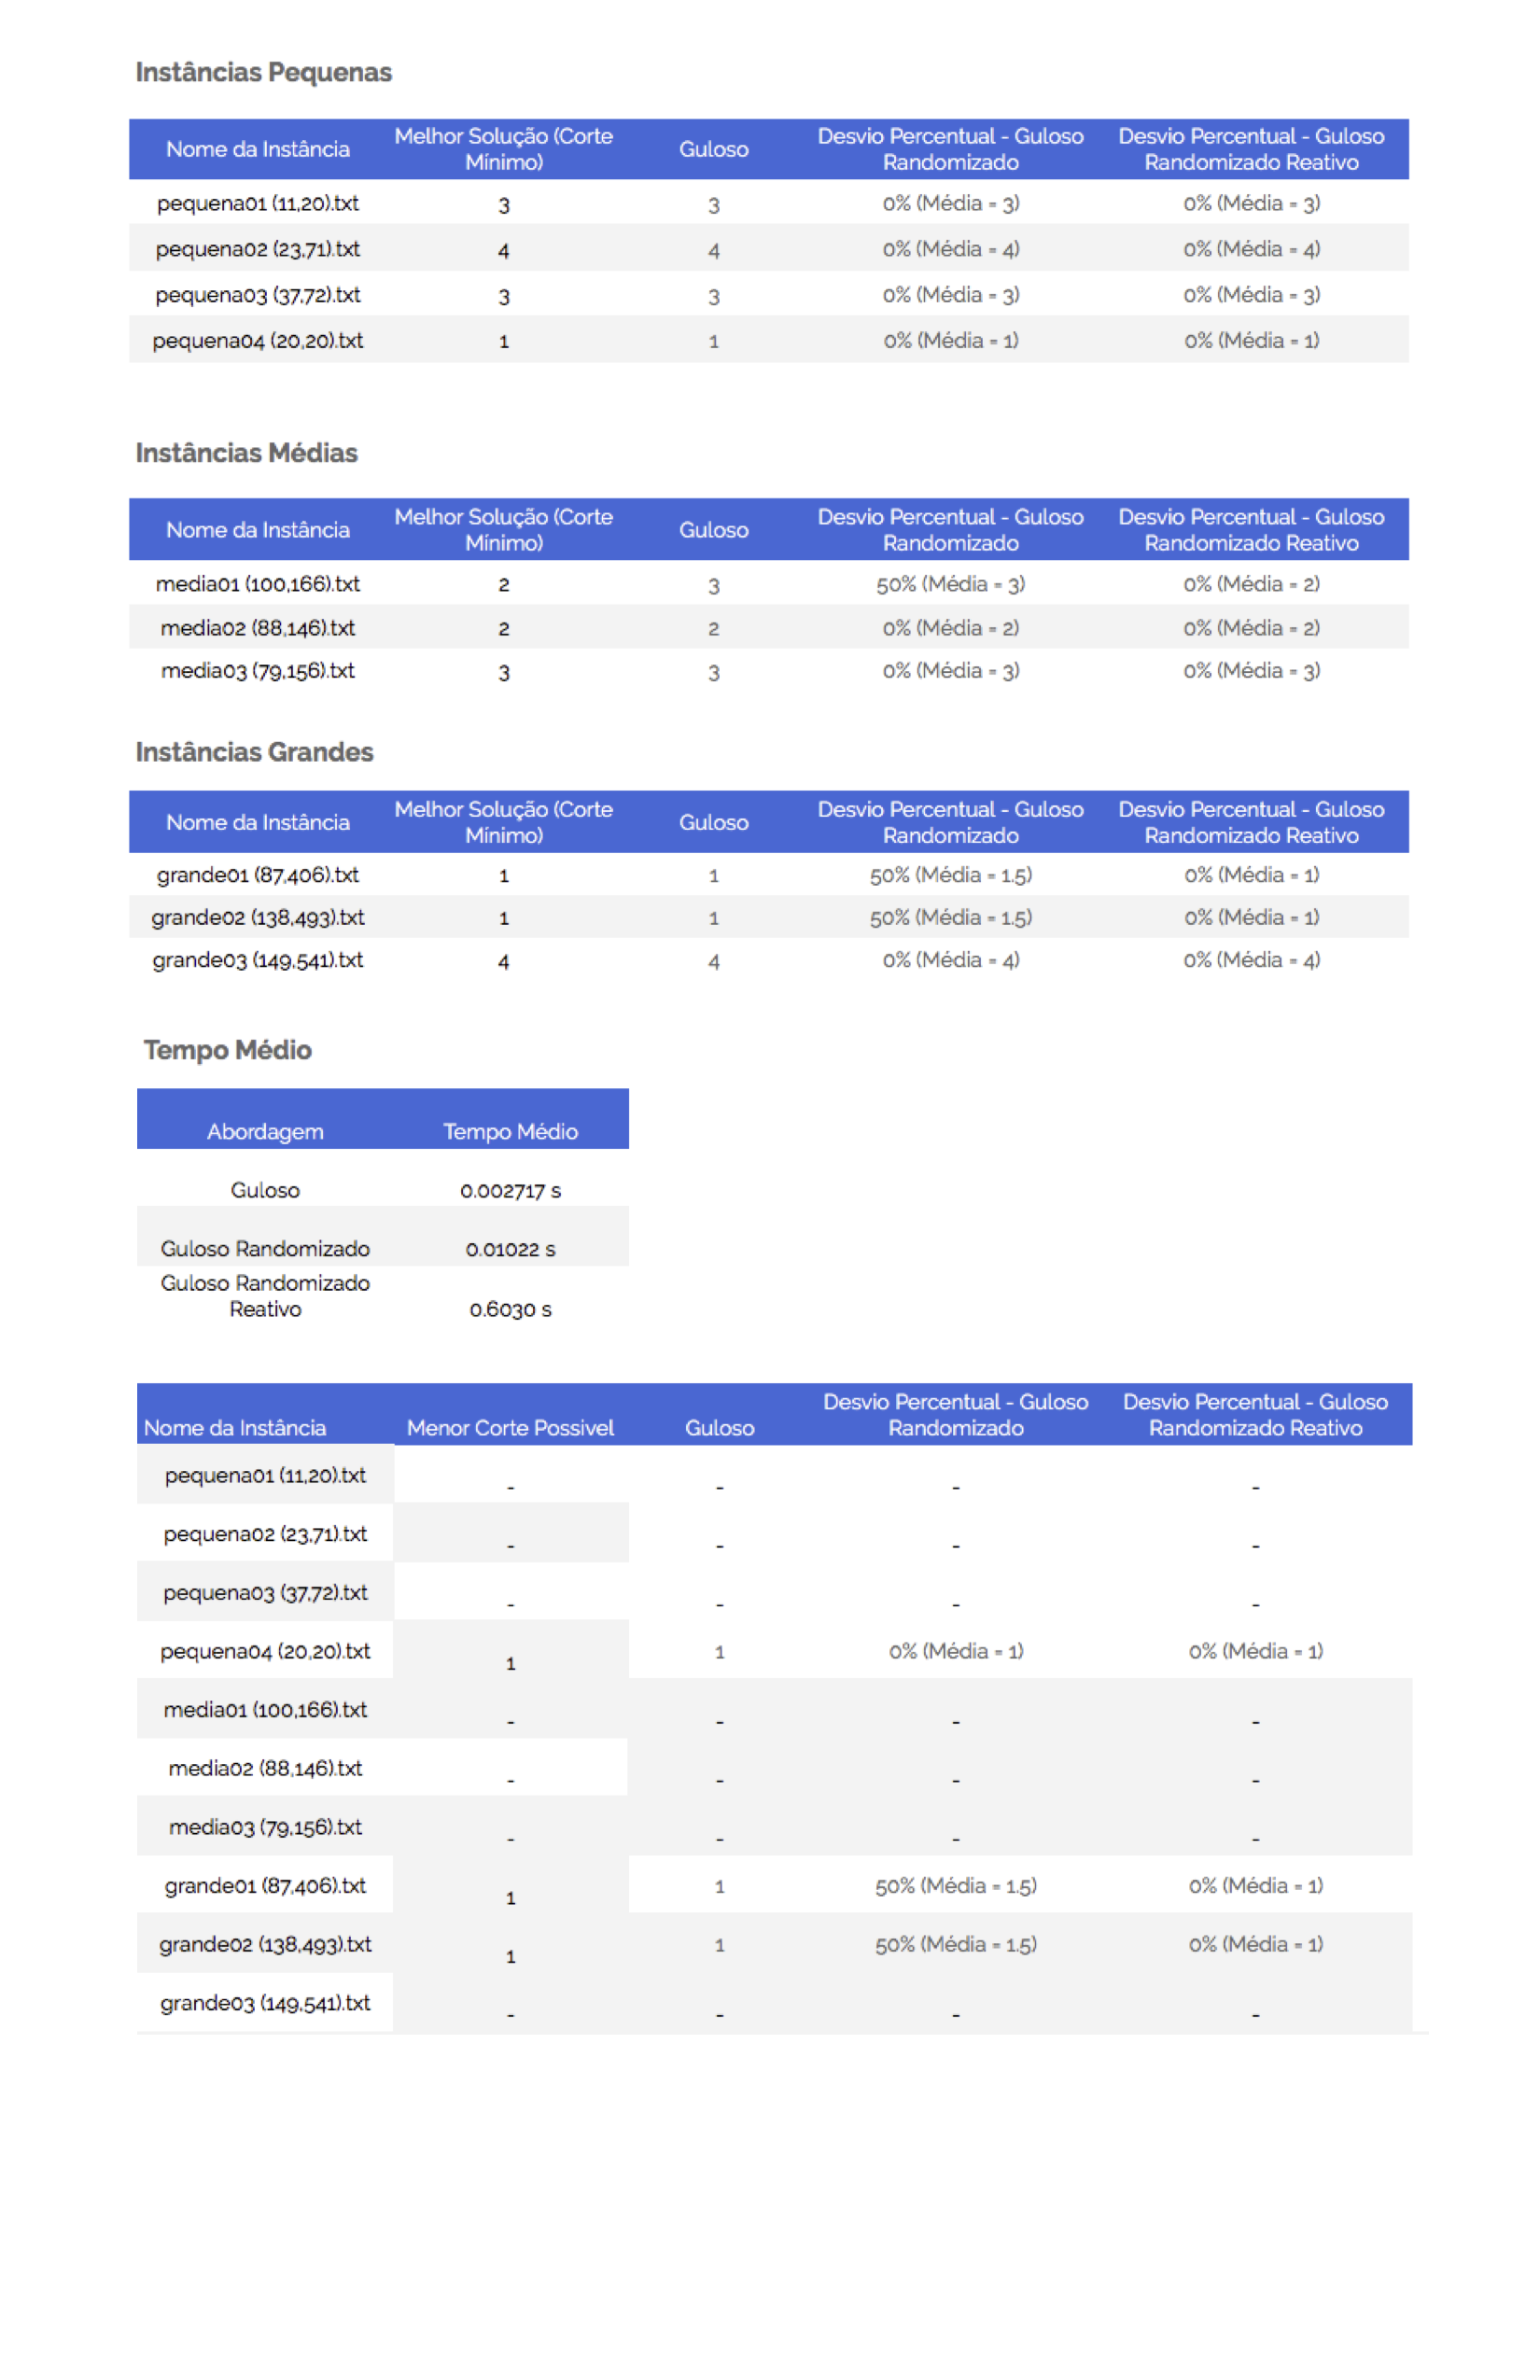
\includegraphics[width=14cm, height = 20cm]{TabelaResultados2}
    \caption{Tabela de com resultados obtidos no segundo teste }
  \end{figure}

\end{document}